%! TEX root = **/010-main.tex
% vim: spell spelllang=en:

\section{Interactive application}%
\label{sec:abi}

As discussed in \cref{sec:structure}, the core of the program is written as a
\emph{C} library which exposes functions through \emph{ABI} (Advanced Binary Interface),
allowing other languages capable of interpreting \emph{C} structures to interact with it
natively. This combined with the really fast computation times makes it really easy to
integrate the functionality of the program into an interactive application to research
how limit cycles behave in a system.
%TODO
%
\subsection{Pluto notebooks}

Pluto notebooks are \emph{Julia} web notebooks designed around the concept of
\emph{javascript} observables, they build a dependency tree between all cells and
if a cell is modified the change propagates to the rest \cite{plas_fonspplutojl_2021}.
This allows to develop
reactive notebooks. \Cref{fig:pluto} shows an example of a \emph{Pluto} notebook
that uses the program to calculate limit cycles with given parameters and
displays the result. Any change in the parameters is propagated and the plot is
updated seamlessly in around 1 second \footnote{With reasonable parameters}.

\begin{figure}[H]
    \centering
    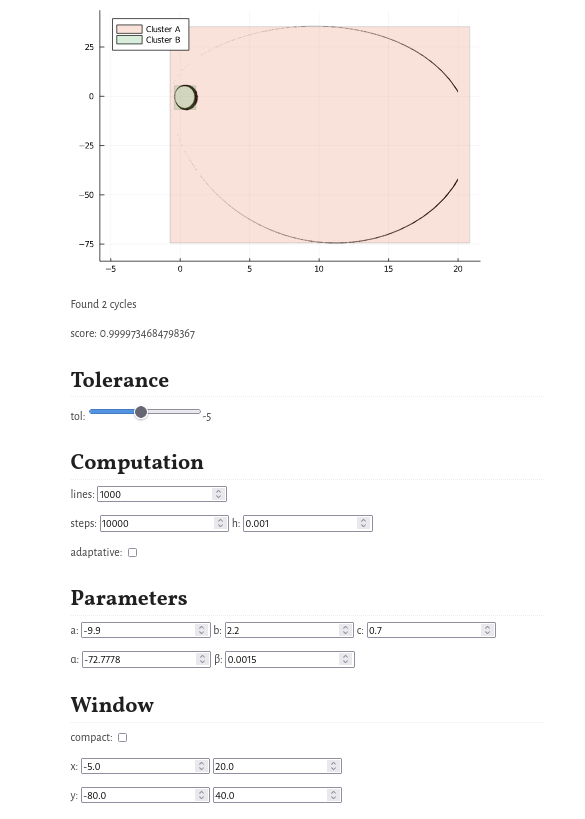
\includegraphics[width=0.4\textwidth]{pluto}
    \caption{Example of interactive Pluto notebook showing 2 limit cycles}%
    \label{fig:pluto}
\end{figure}

\subsection{OpenGL}

Another useful feature is the interoperability between \emph{CUDA} and
\emph{OpenGL}, allowing to bind the actual data used in \emph{CUDA} in the GPU
to \emph{OpenGL} textures which can be rendered directly to the screen
\cite{noauthor_opengl_nodate}. Using little modification to the program
an interactive render of the GPU data can be done.

\begin{figure}[H]
    \centering
    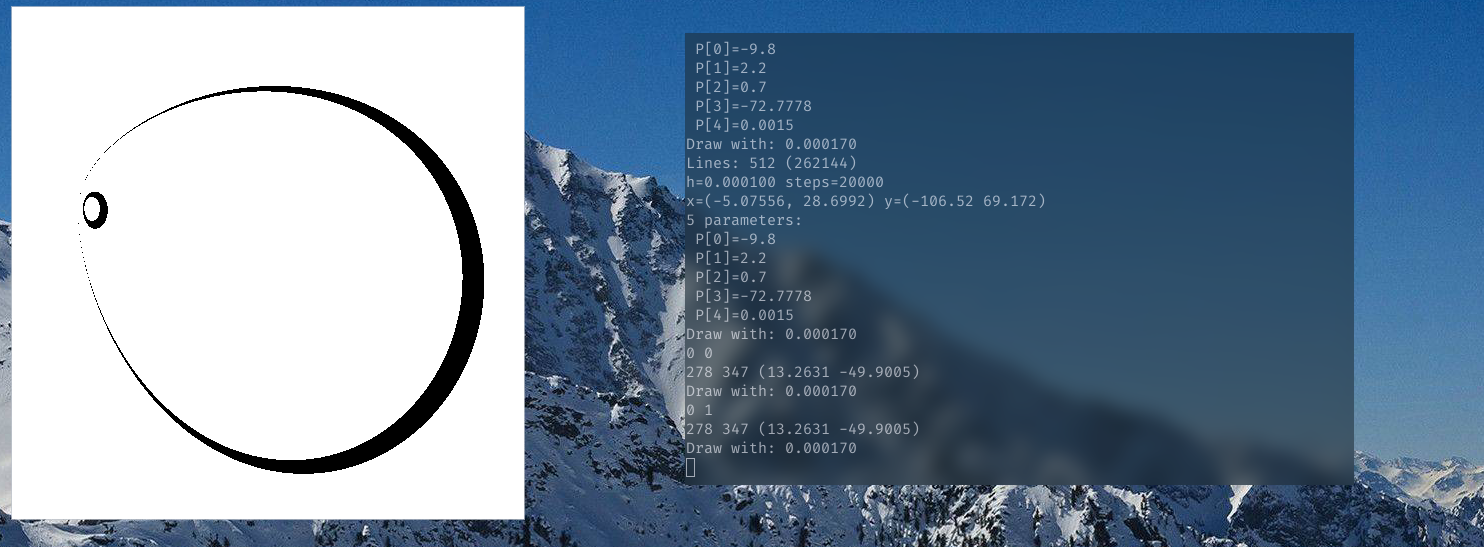
\includegraphics[width=0.8\textwidth]{opengl}
    \caption{OpenGL window directly displaying CUDA results}%
    \label{fig:opengl}
\end{figure}

\subsection{CUDA limitations on interactivity}

One of the main problems with the current implementation is that changing the system
involves creating a new \emph{CUDA} function and recompiling the library, this makes
using the program as a library quite challenging since the use must know how to
program the function and compile it. Without using \emph{CUDA} we could simply
use function pointers so that any arbitrary function can be passed and no need
for recompilation is needed. However, function pointers are extremely slow in \emph{CUDA}
since the function cannot be \emph{inlined} and we introduce massive overhead by
adding function calls to the stack.

One option is to implement a program to parse ODE systems with a strict syntax,
produces the \emph{CUDA} kernel compiles it and dynamically links it to the
program. It should be possible to do from \emph{Julia}.
